\section{Fairness in bipartite ranking}

\subsection{Motivation}
\begin{frame}{Motivation}
    \begin{itemize}
        \item Most of \gbf{fairness-aware} machine learning research focuses on \gbf{classification} models.
        \item Because bipartite ranking models are evaluated differently (\textit{i.e}, with ROC curves), evaluating fairness for bipartite ranking models might be \gbf{more challenging}.        
        \item However, learning a scoring function over a classifier adds \gbf{more flexibility} to the thresholds, which means that a fair scoring function will lead to \gbf{fair decisions for all thresholds of interest}.
    \end{itemize}
\end{frame}


\subsection{AUC-based constraints}
\begin{frame}{AUC-based constraints}
    
    Previous works proposed to use \gbf{AUC-based constraints} to ensure fairness in bipartite ranking models. Let's denote $G_s^{(i)}$ (resp. $H_s^{(i)}$) the CDF of the score on the positive (resp. negatives) of group $z \in \{0,1\}$.
    
    \citeauthor{beutel2019fairness}\footcite{beutel2019fairness} proposed to use \gbf{intra-group pairwise} AUC fairness :
    \begin{equation}
        AUC_{H_s^{(0)},G_s^{(0)}} = AUC_{H_s^{(1)},G_s^{(1)}}
    \end{equation}

\end{frame}


\begin{frame}{AUC-based constraints}
    
    \citeauthor{borkan2019nuanced}\footcite{borkan2019nuanced} proposed to use \gbf{Background Negative Subgroup Positive (BNSP)} AUC fairness :

    \begin{equation}
        AUC_{H_s,G_s^{(0)}} = AUC_{H_s,G_s^{(1)}}
    \end{equation}
    
    Finally, \citeauthor{kallus2019fairness}\footcite{kallus2019fairness} proposed to use \gbf{inter-group pairwise} AUC fairness :

    \begin{equation}
        AUC_{H_s^{(0)},G_s^{(1)}} = AUC_{H_s^{(1)},G_s^{(0)}}
    \end{equation}

\end{frame}
    

\begin{frame}{AUC-based constraints}


    {\large\textbf{What is the difference ?}}
    \begin{itemize}
        \item \textbf{Intra-group fairness} : equal performance \gbf{within} groups
        \item \textbf{Background Negative Subgroup Positive fairness} : positives \gbf{from either
        group} have the \gbf{same probability of being ranked higher} than a negative example
        \item \textbf{Inter-group fairness} (in this specific case) : positives of a group can be distinguished from the \gbf{negatives of the other group} as effectively for both groups
    \end{itemize}


\end{frame}


\begin{frame}{AUC-based constraints}
    There are \gbf{many more constraints} available !\footnote{If you're interested, check out the supplementary material of the original paper}. This is one of the \gbf{strengths} of the method proposed by the authors : \gbf{it can be adapted to any fairness constraint} we might be interested in thanks to the following framework :

    \begin{align} \label{eq:auc-based-constraints-general}
        AUC_{\alpha^\top D(s), \beta^\top D(s)} = AUC_{\alpha'^\top D(s),
        \beta'^\top D(s)}.
    \end{align}

    with $ D(s) := (H^{(0)}_s, H^{(1)}_s, G^{(0)}_s, G^{(1)}_s)^\top$ and the probability vectors $\alpha, \beta, \alpha', \beta' \in  \mathcal{P}$ where $\mathcal{P} = \{ v \mid v \in \mathbf{R}_+^4, \mathbf{1}^\top v = 1 \}$.

\end{frame}


\begin{frame}{AUC-based constraints}
    Equation \ref{eq:auc-based-constraints-general} is under-specified, so the authors finally formulate all relevant constraints as a linear combination of 5 elementary constraints.

    \vspace{-0.85cm} 
    \begin{align*}
        C_1(s) &= AUC_{H^{(0)}_s, H^{(1)}_s} - 1/2,\\
        C_2(s) &=   1/2 - AUC_{G^{(0)}_s, G^{(1)}_s},\\
        C_3(s) &= AUC_{H^{(0)}_s, G^{(0)}_s} - AUC_{H^{(0)}_s, G^{(1)}_s}, \\
        C_4(s) &= AUC_{H^{(0)}_s, G^{(1)}_s} - AUC_{H^{(1)}_s, G^{(0)}_s}, \\
        C_5(s) &= AUC_{H^{(1)}_s, G^{(0)}_s} - AUC_{H^{(1)}_s, G^{(1)}_s}.
    \end{align*}


    The family of fairness constraints we consider is then the set of linear
    combinations of the $C_l(s) = 0$:
    \begin{align}\label{eq:barycenter-constraint-formulation}
        \mathcal{C}_\Gamma(s): \quad \Gamma^\top C(s) &= \textstyle\sum_{l=1}^5
        \Gamma_l C_l (s) = 0,
    \end{align}

    where $\Gamma = (\Gamma_1 , \dots, \Gamma_5)^\top \in \mathbf{R}^5$.


\end{frame}



\begin{frame}{Limits of AUC-based constraints}
    \begin{columns}
        \begin{column}{0.5\textwidth}
            \begin{figure}[t]
                \centering
                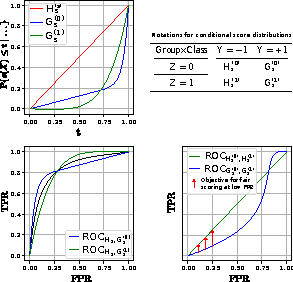
\includegraphics[width=1\columnwidth, trim = 0cm 0cm 2.35cm 2.4cm, clip]{images/original_paper/example_simple_dists_explained_with_table2.pdf}
                \caption{Illustrating the limitations of $AUC$-based fairness.}
                \label{fig:example-1}
            \end{figure}
        \end{column}

        \begin{column}{0.5\textwidth}
            \begin{itemize}
                \item Here, both AUCs are equal.
                \item However, when looking at the beginning, there are a lot more false positives for the sensitive group.
            \end{itemize}
        \end{column}
    \end{columns}
    
\end{frame}

\subsection{ROC based constraints}
\begin{frame}{ROC based constraints}
    
\end{frame}
